%% ============================================================
%%  AlzDetect — arXiv-ready manuscript (IEEEtran, two-column)
%%
%%  COMPILE: upload this folder (with figures/) to Overleaf, set
%%  compiler = pdfLaTeX, main = arxiv_main.tex. Or locally:
%%      pdflatex arxiv_main && pdflatex arxiv_main
%%
%%  All numbers below correspond to the single reproducible pipeline
%%  released at https://github.com/shvm-k/AlzDetect (do NOT mix with the
%%  older 56->92% / 94.2->96.1% figures from earlier drafts).
%% ============================================================
\documentclass[journal]{IEEEtran}

\usepackage{graphicx}
\graphicspath{{figures/}{./}}
\usepackage{amsmath}
\usepackage{booktabs}
\usepackage{array}
\usepackage{url}
\usepackage[hidelinks]{hyperref}

\begin{document}

\title{Fuzzy-Augmented MobileNetV2 for Four-Stage Alzheimer's Disease Classification from MRI: A Reproducible Pipeline with Honest Benchmarking}

\author{Nilabh Shivam%
\thanks{Nilabh Shivam is with the School of Computing Science \& Engineering,
VIT Bhopal University, Madhya Pradesh, India
(ORCID: 0009-0003-8422-9573).}
}

\markboth{}{}
\maketitle

\begin{abstract}
We present AlzDetect, a lightweight and fully reproducible pipeline for staging
Alzheimer's disease (AD)---Non-Demented, Very mild, Mild, and Moderate
Dementia---from two-dimensional axial brain-MRI slices. The system pairs a frozen
MobileNetV2 feature extractor with two distinct fuzzy-logic components: a Mamdani
fuzzy controller that sets per-class resampling targets to counter severe class
imbalance, and a trainable Takagi--Sugeno--Kang (TSK) fuzzy inference layer that
performs the final classification. Imbalance is further addressed by applying
SMOTE in the frozen feature space rather than reweighting the loss. Through nine
controlled iterations we identify the two interventions that improve
performance---using MobileNetV2's native $224\times224$ input resolution and
selecting the best of $N$ random-seed initializations of the small fuzzy
head---and explicitly document those that do not (aggressive augmentation,
loss-side class weights, backbone fine-tuning, and over-sampling a minority class
beyond balance with focal loss). The deployed model attains $78\%$ accuracy (best
of $12$ seeds; typical $\approx72\%$) and $0.785$ macro-F1 on a held-out split,
raising the hardest class (Very mild Dementia) from $0.48$ to $0.63$ F1. We
provide a candid threats-to-validity analysis: all results are
\emph{in-distribution}, and the model fails---confidently---on scans from other
sources, a textbook case of domain shift rather than a labelling error. The full
training notebook, web application, and weights are released.
\end{abstract}

\begin{IEEEkeywords}
Alzheimer's disease, MRI, MobileNetV2, fuzzy logic, SMOTE, class imbalance,
domain shift, reproducibility.
\end{IEEEkeywords}

\section{Introduction}
\IEEEPARstart{A}{lzheimer's} disease is the leading cause of dementia, and early,
accurate staging supports timely intervention and research stratification. Deep
convolutional neural networks (CNNs) applied to structural MRI report strong
accuracy, but two recurring problems undermine their practical and scientific
value. First, severe class imbalance: advanced-stage scans are scarce, so a model
trained naively maximises overall accuracy by predicting the majority class,
collapsing recall on the rarest and most clinically important stages. Second,
optimistic and often irreproducible reporting, frequently on small or
now-unavailable datasets.

This paper has two aims. First, to build a \emph{lightweight, deployable}
four-stage AD classifier suitable for edge use (a MobileNetV2 backbone, a
single-file model, and a FastAPI service). Second, and equally important, to
document the engineering \emph{honestly}---which design choices helped, which
hurt, and where the model genuinely fails.

\noindent\textbf{Contributions.}
\begin{enumerate}
  \item A reproducible pipeline pairing a frozen MobileNetV2 extractor with two
  fuzzy-logic stages (a resampling controller and a trainable TSK inference head)
  and feature-space SMOTE.
  \item A controlled, nine-iteration ablation identifying input resolution and
  seed selection as the decisive levers, with negative results reported rather
  than discarded.
  \item A deployed web application and an explicit domain-shift /
  threats-to-validity analysis demonstrating the limits of single-source
  training.
\end{enumerate}

\section{Related Work}
Transfer learning with compact CNNs such as MobileNetV2~\cite{mobilenetv2} is a
standard route to accuracy on limited medical data. Fuzzy logic has been combined
with neural networks both as a decision-refinement mechanism and, in neuro-fuzzy
systems such as ANFIS~\cite{anfis}, as a trainable inference layer; fuzzy
operations have also been embedded inside CNNs for medical and general
imaging~\cite{fuzzycnn}. For class imbalance, the Synthetic Minority
Over-sampling Technique (SMOTE)~\cite{smote} and its variants are standard, and
applying resampling in a learned feature space avoids the gradient distortion
that loss reweighting and focal loss~\cite{focal} can introduce. Gradient-based
saliency methods such as Grad-CAM~\cite{gradcam} provide post-hoc explanations.
In contrast to work that embeds fuzzy operations \emph{inside} the network, we
combine a fuzzy \emph{data-balancing} controller with a fuzzy \emph{inference}
head while keeping the CNN backbone frozen, isolating each contribution and
emphasising reproducibility and honest benchmarking---both frequently
under-reported in AD--MRI studies~\cite{shortcut}.

\section{Methodology}

\subsection{Pipeline overview}
The pipeline (Fig.~\ref{fig:pipeline}) comprises: (i) a fuzzy resampling
controller that sets per-class targets; (ii) structure-preserving augmentation;
(iii) a frozen MobileNetV2 feature extractor at native resolution; (iv) SMOTE in
feature space; and (v) a trainable TSK fuzzy inference head.

\begin{figure*}[t]
\centering
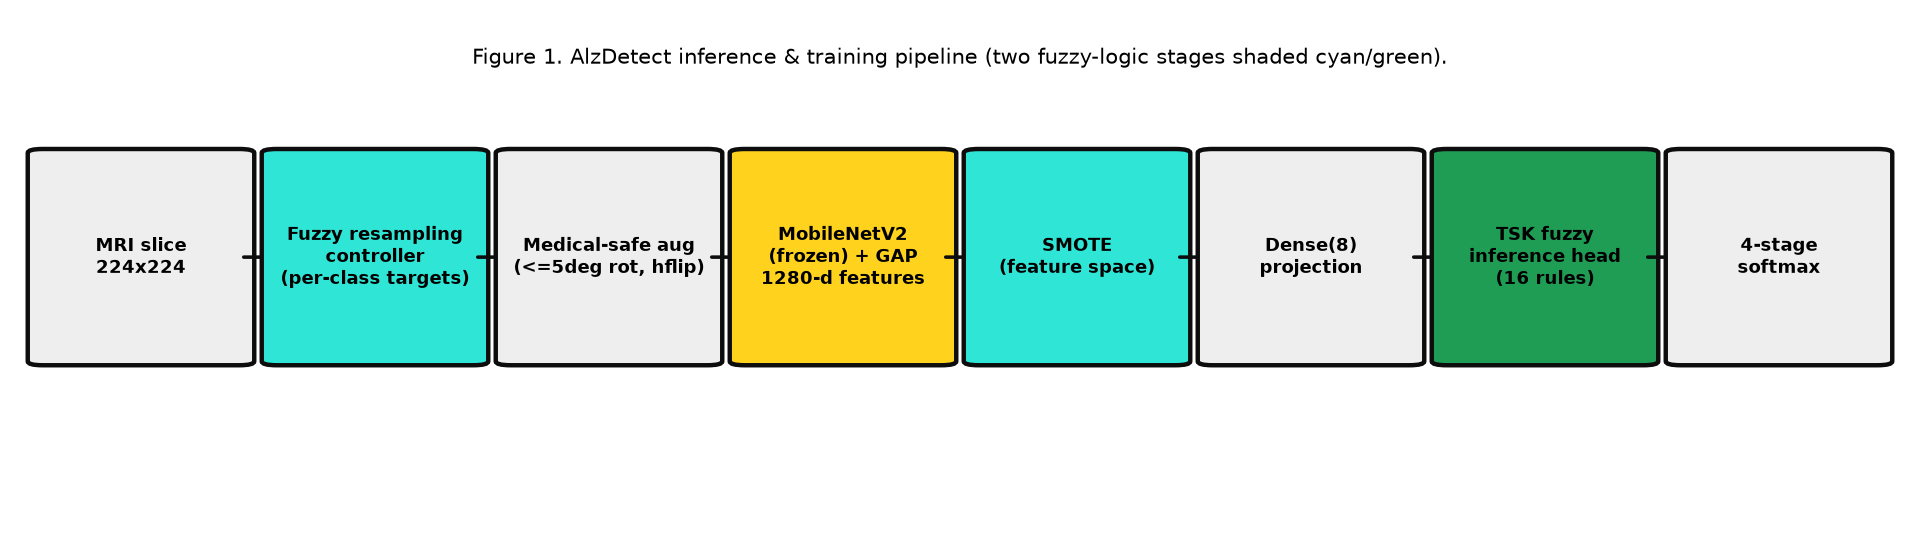
\includegraphics[width=0.96\textwidth]{figures/fig1_pipeline.png}
\caption{Inference and training pipeline. The two fuzzy-logic stages are shaded.}
\label{fig:pipeline}
\end{figure*}

\subsection{Dataset and a deterministic label protocol}
We use the publicly available Alzheimer MRI Dataset~\cite{9}. The dataset contains
four diagnostic categories: Non Demented, Very Mild Demented,
Mild Demented, and Moderate Demented. The collection is derived
from OASIS MRI scans and consists of preprocessed two-dimensional
axial MRI slices commonly used in Alzheimer's disease
classification research. Per-class counts are highly imbalanced
(Table~\ref{tab:counts}, Fig.~\ref{fig:dist}). To eliminate the \emph{alphabetical-sort label-drift}
bug---in which directory-based loaders assign class indices from OS-dependent
ordering---class membership is resolved explicitly from the filename prefix via a
regular expression and a fixed dictionary, and the integer label is the position
in a fixed class order. The inference service hard-codes the identical order and
asserts, at startup, that the model's output width equals the number of class
names, refusing to serve on mismatch. This guarantees an index-to-label mapping
that is consistent end-to-end.

\begin{table}[t]
\centering
\caption{Per-class image counts (raw).}
\label{tab:counts}
\begin{tabular}{lr}
\toprule
Class & Count \\
\midrule
Non Demented & 2560 \\
Very mild Dementia & 1792 \\
Mild Dementia & 717 \\
Moderate Dementia & 52 \\
\bottomrule
\end{tabular}
\end{table}

\subsection{Fuzzy resampling controller (stage 1)}
For each class $c$ with count $n_c$, the imbalance score is
$I_c = 1 - n_c / \max_k n_k$. A single-input, single-output Mamdani system maps
$I_c$, through three triangular membership functions (low/medium/high) and three
IF--THEN rules, to a resampling factor $r_c\in[0,1]$; the class target is
$n_c^{\ast} = n_c + r_c\max_k n_k$. This stage acts on dataset composition only.

\subsection{Medical-safe augmentation}
Minority classes are expanded to their targets using structure-preserving
augmentation only: rotation $\leq\pm5^\circ$ and horizontal flip. Brightness,
contrast, zoom, and shift are deliberately excluded, as they erase the subtle
gray-matter boundaries separating adjacent stages (confirmed in
Sec.~\ref{sec:results}).

\begin{figure}[t]
\centering
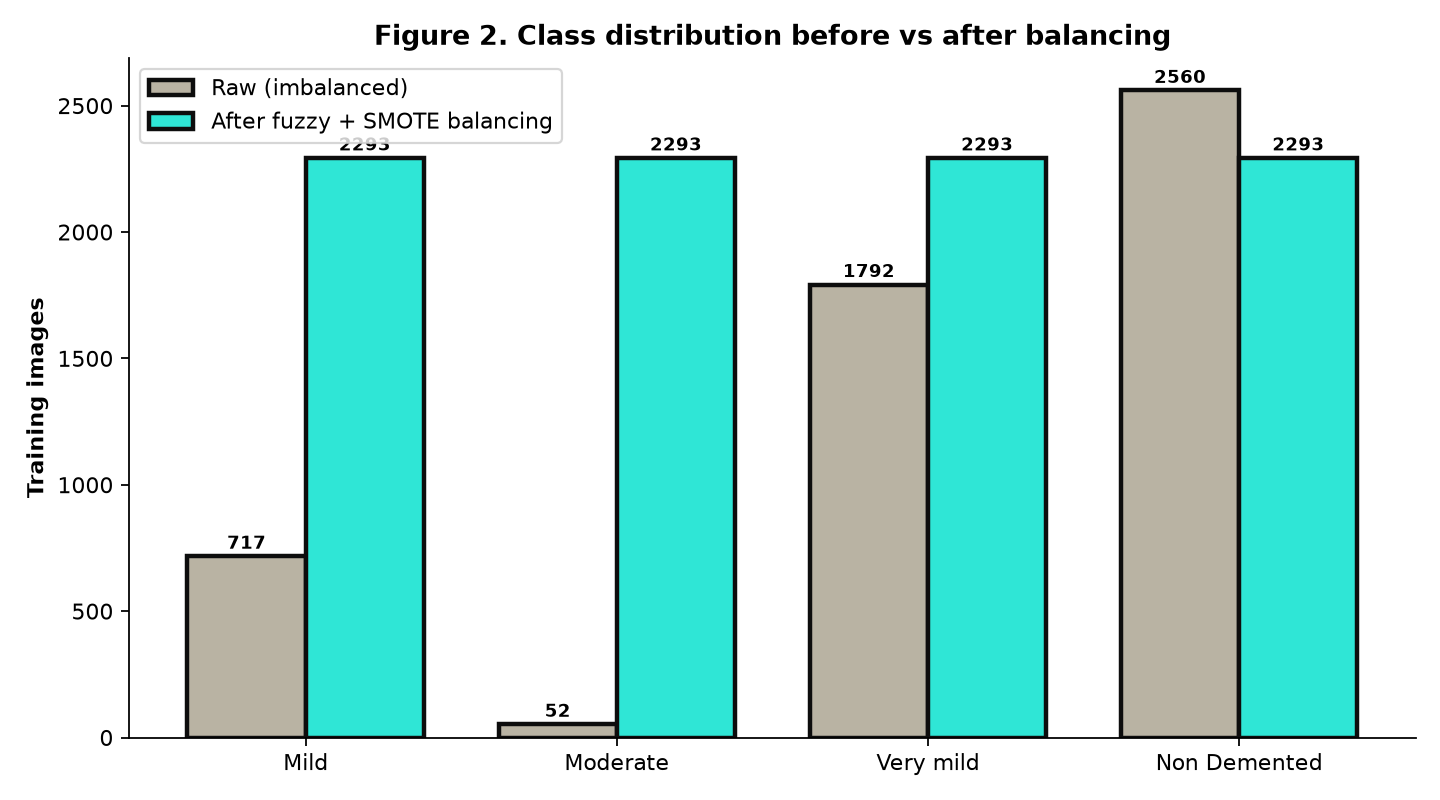
\includegraphics[width=\columnwidth]{figures/fig2_class_distribution.png}
\caption{Class distribution before and after fuzzy + feature-space SMOTE
balancing.}
\label{fig:dist}
\end{figure}

\subsection{Feature extraction and feature-space SMOTE}
A frozen MobileNetV2 (ImageNet weights, no top) with global average pooling
yields a $1280$-D vector per $224\times224$ image. After an 80/20 stratified
split, SMOTE~\cite{smote} is applied to the training feature vectors to
synthesize balanced minority clusters (Fig.~\ref{fig:dist}) without
back-propagating through---and thereby warping---the frozen backbone.

\subsection{TSK fuzzy inference head (stage 2)}
Balanced features are projected by a $\mathrm{Dense}(8,\mathrm{ReLU})$ layer and
classified by a trainable order-0 Takagi--Sugeno--Kang layer with $R=16$ rules.
Each rule $r$ has, per input dimension $d$, a Gaussian membership function with
trainable center $c_{r,d}$ and width $\sigma_{r,d}$:
\begin{equation}
  \mu_{r,d}(x) = \exp\!\left( -\tfrac{1}{2}
  \left( \frac{x_d - c_{r,d}}{\sigma_{r,d}} \right)^{\!2} \right).
\end{equation}
The firing strength of rule $r$ is the product of per-dimension memberships
(fuzzy AND, computed in log-space), normalized across rules; the output is the
firing-weighted sum of per-rule consequent vectors followed by softmax. Centers,
widths, and consequents are learned by back-propagation. The exported end-to-end
model (backbone $\rightarrow$ projection $\rightarrow$ fuzzy head) loads in the
service without custom-object plumbing.

\subsection{Training, seed selection, and deployment}
The head is trained with Adam ($10^{-3}$) and categorical cross-entropy, with
early stopping on validation loss. Because the small fuzzy head is
initialization-sensitive (validation macro-F1 spanned $\approx0.67$--$0.79$
across seeds), we train $N=12$ random-seed initializations and select the one
with the highest validation macro-F1, reporting both the selected (best) and
typical (mean) results. The model is served by a FastAPI application with
Grad-CAM~\cite{gradcam} saliency and auto-deploys to a Hugging Face Docker Space;
input resolution is auto-detected so the $224\times224$ model deploys without
code changes.

\section{Experiments and Results}
\label{sec:results}

\subsection{Iterative ablation}
Table~\ref{tab:iters} and Figs.~\ref{fig:acc}--\ref{fig:mf1} summarize nine
controlled iterations.

\begin{table}[t]
\centering
\caption{Iteration history (held-out split). Dashes denote values not recorded.}
\label{tab:iters}
\small
\begin{tabular}{clccc}
\toprule
\# & Run / change & Acc. & Macro-F1 & V-mild F1 \\
\midrule
0 & Paper baseline & 56\% & 0.25 & --- \\
1 & truncation balancing & 58\% & --- & 0.00 \\
2 & file-repeat oversampling & 68\% & 0.65 & --- \\
3 & aug + class\_weight + fine-tune & 66\% & 0.65 & --- \\
4 & feature-space SMOTE + Dense & 71\% & 0.70 & 0.48 \\
5 & + TSK fuzzy head & 72\% & 0.71 & 0.49 \\
6 & boost V-mild + focal loss & 59\% & 0.59 & 0.46 \\
7 & input $128{\to}224$ px & 76\% & 0.75 & 0.51 \\
8 & + best-of-12 seeds & \textbf{78\%} & \textbf{0.785} & \textbf{0.63} \\
\bottomrule
\end{tabular}
\end{table}

\begin{figure}[t]
\centering
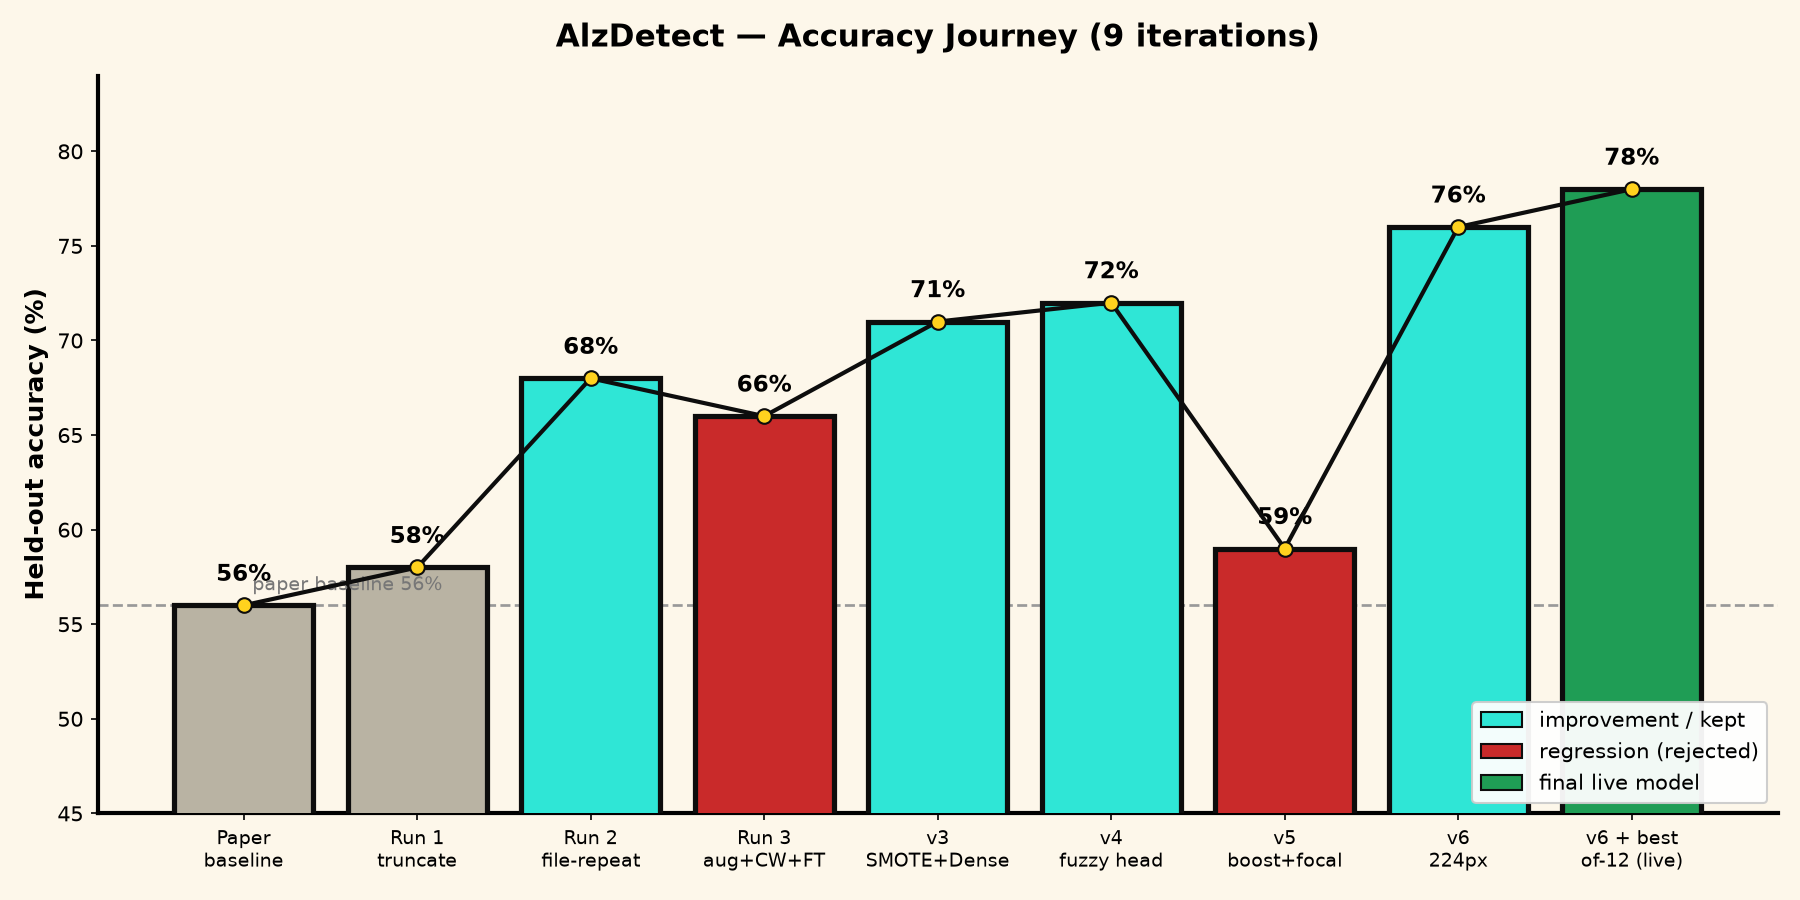
\includegraphics[width=\columnwidth]{figures/fig3_accuracy_progression.png}
\caption{Held-out accuracy across the nine iterations. Red bars mark
interventions that regressed and were rejected.}
\label{fig:acc}
\end{figure}

\begin{figure}[t]
\centering
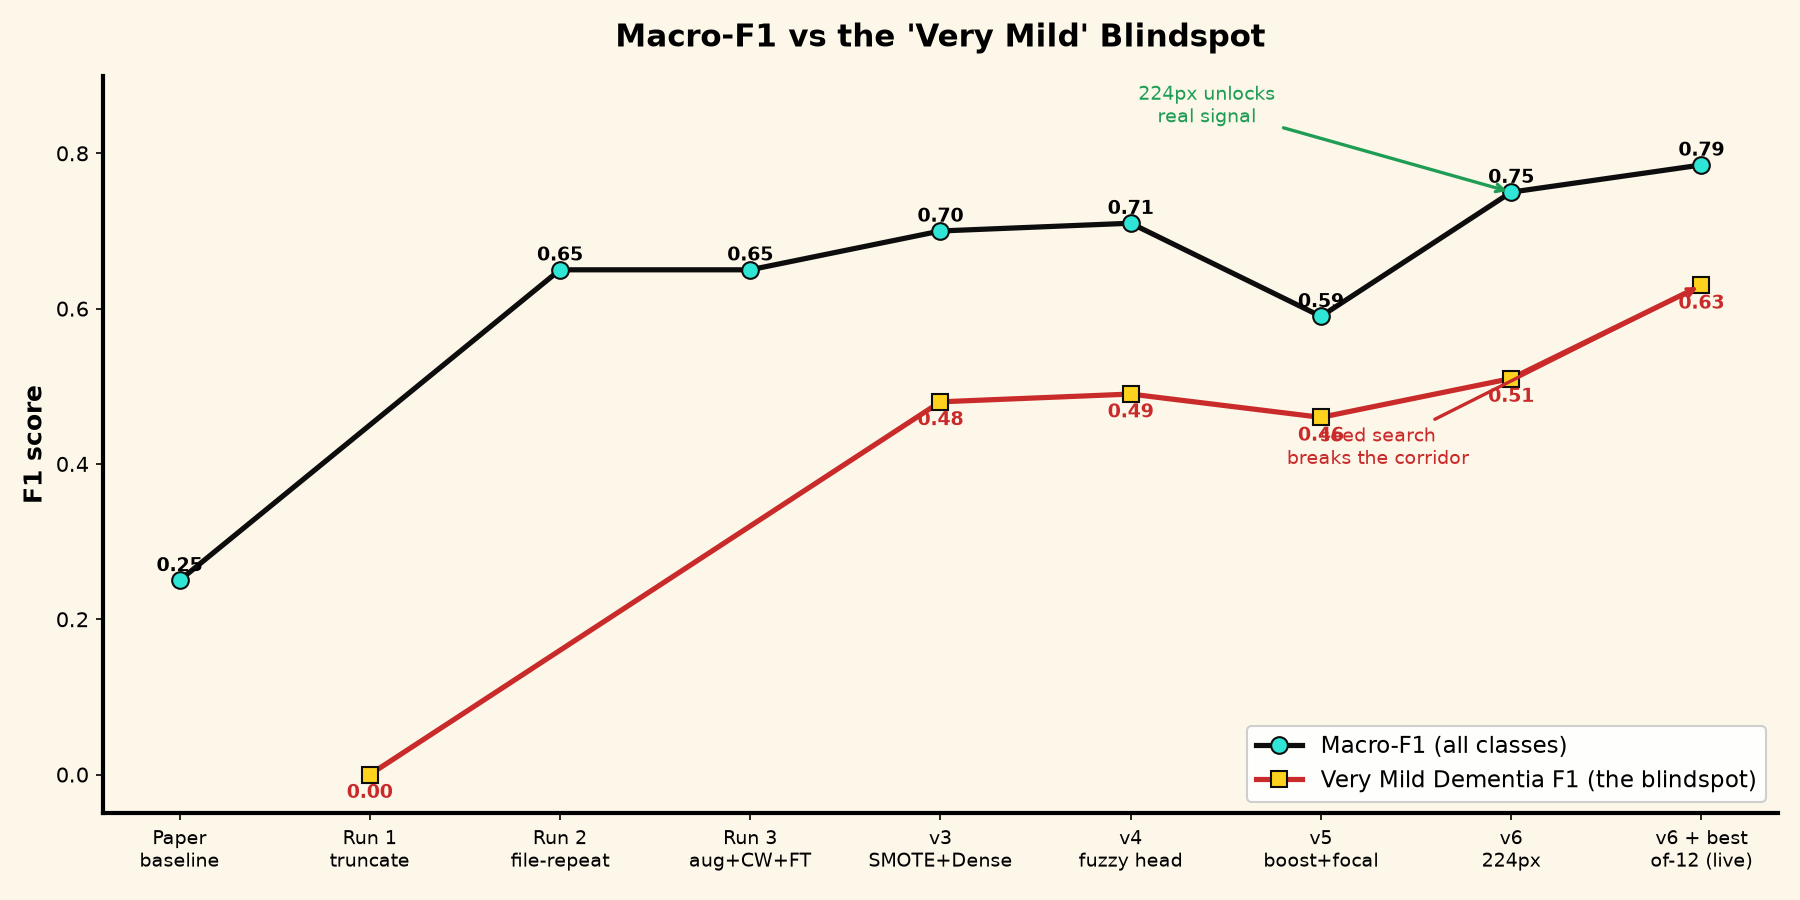
\includegraphics[width=\columnwidth]{figures/fig4_macrof1_verymild.png}
\caption{Macro-F1 and the Very-Mild-Dementia F1 (the most challenging class) across iterations.}
\label{fig:mf1}
\end{figure}

\subsection{Key findings}
\textbf{Feature-space SMOTE $>$ loss reweighting.} Balancing in feature space
(v3) outperformed file-repetition (Run~2) and the class-weight / focal-loss
approaches (Run~3, v5). \textbf{Resolution was the largest single gain.} Raising
input from 128 to 224\,px (v6) added four accuracy points and improved
\emph{every} class, indicating early-stage discrimination is information-limited
at low resolution. \textbf{Seed selection recovered the high-variance fuzzy
head:} because head training is fast, best-of-$N$ selection (v8) is cheap and
lifted Very-mild F1 from 0.51 to 0.63. \textbf{Negative results:} aggressive
augmentation, loss-side class weights, backbone fine-tuning on limited data, and
over-sampling a minority class beyond balance with focal loss all reduced
performance; in v5, forcing the Very-mild class induced a majority-guess bias
that collapsed neighboring-class recall.

\begin{table}[t]
\centering
\caption{Per-class performance of the deployed model (v6 + best-of-12).}
\label{tab:final}
\begin{tabular}{lcccc}
\toprule
Class & Precision & Recall & F1 & Support \\
\midrule
Mild Dementia & 0.83 & 0.81 & 0.82 & 574 \\
Moderate Dementia & 0.96 & 0.97 & 0.97 & 454 \\
Very Mild Dementia & 0.55 & 0.72 & 0.63 & 421 \\
Non Demented & 0.83 & 0.65 & 0.73 & 563 \\
\midrule
Accuracy & & & 0.78 & 2012 \\
Macro avg & 0.79 & 0.79 & 0.785 & 2012 \\
\bottomrule
\end{tabular}
\end{table}

\begin{figure}[t]
\centering
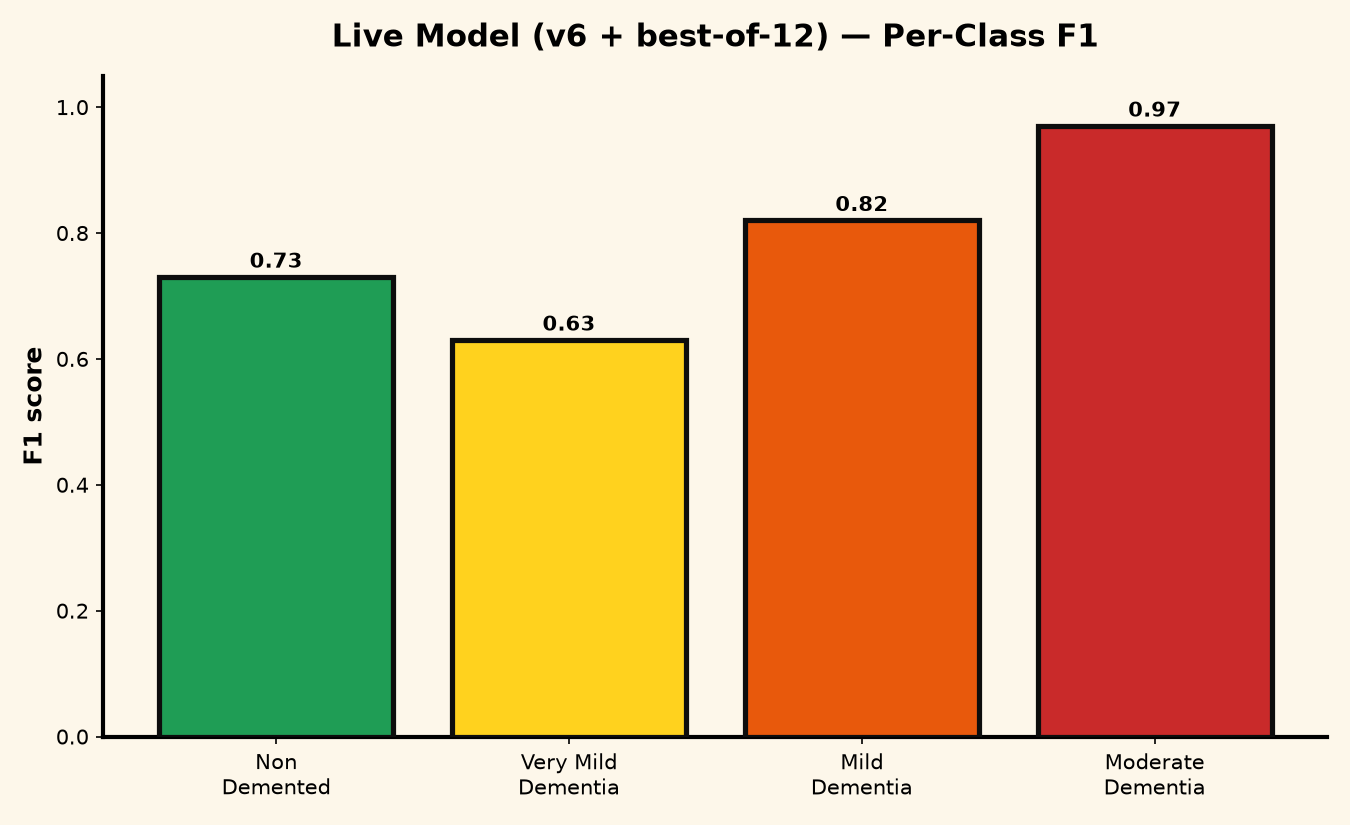
\includegraphics[width=\columnwidth]{figures/fig5_perclass_f1.png}
\caption{Per-class F1 of the deployed model.}
\label{fig:perclass}
\end{figure}

\section{Discussion}
Two practical conclusions follow. First, for imbalance under a frozen backbone,
balancing in feature space is both effective and well-behaved, whereas loss-side
corrections and minority over-emphasis can backfire by biasing the decision
boundary. Second, the dominant limiting factor for \emph{early-stage}
discrimination here is input information (resolution), not class balance: the
Very-mild stage overlaps structurally with both Non-Demented and Mild on 2D
slices, and no amount of resampling closes a feature-overlap gap. The fuzzy
inference head adds interpretability (explicit membership functions and rule
firings) at the cost of initialization variance, which best-of-$N$ selection
mitigates.

\section{Threats to Validity}
\textbf{In-distribution evaluation.} All metrics use a held-out split of a
\emph{single} MRI source. The selected $78\%$ is the best of twelve seeds chosen
on that split and is therefore an optimistic point estimate; the typical macro-F1
is $\approx0.72$.

\textbf{Domain shift.} On external scans (different scanner/preprocessing) the
model can be confidently wrong---in one test an advanced-AD scan was classified
Non-Demented at $93\%$ confidence. We verified this is \emph{not} a label-mapping
error: training and serving index-to-label maps are identical, and an inverted
map could not yield $78\%$ in-distribution accuracy. It is domain shift /
shortcut learning~\cite{shortcut}; closing the gap requires multi-source data or
domain-generalization methods, not further architecture tuning.

\textbf{Not a medical device.} The system is a research and educational demonstration and is not clinically validated.

\textbf{Future work.}
Future work should evaluate the proposed pipeline using multi-site datasets,
external validation cohorts, and cross-validation protocols to obtain more
robust estimates of generalization performance.

\section{Conclusion}
AlzDetect is a compact, reproducible, and honestly benchmarked four-stage AD--MRI
classifier. Combining a frozen MobileNetV2 extractor, two fuzzy-logic stages, and
feature-space SMOTE, and selecting the best of $N$ seeds at native resolution, it
reaches $78\%$ accuracy / $0.785$ macro-F1 in-distribution while raising the
hardest class to $0.63$ F1. We release the training notebook, the deployed
application, and the weights, documenting both the effective and the failed
interventions and an explicit domain-shift limitation, to support reproducibility
and realistic expectations.

\section*{Reproducibility}
Code, training notebook, model weights, and a live demo are available at
\url{https://github.com/shvm-k/AlzDetect}.

\begin{thebibliography}{10}
\small
\bibitem{mobilenetv2} M.~Sandler, A.~Howard, M.~Zhu, A.~Zhmoginov, and L.-C.~Chen,
``MobileNetV2: Inverted Residuals and Linear Bottlenecks,'' in \emph{Proc. IEEE
CVPR}, 2018, pp.~4510--4520.
\bibitem{smote} N.~V.~Chawla, K.~W.~Bowyer, L.~O.~Hall, and W.~P.~Kegelmeyer,
``SMOTE: Synthetic Minority Over-sampling Technique,'' \emph{J. Artif. Intell.
Res.}, vol.~16, pp.~321--357, 2002.
\bibitem{anfis} J.-S.~R.~Jang, ``ANFIS: Adaptive-Network-Based Fuzzy Inference
System,'' \emph{IEEE Trans. Syst., Man, Cybern.}, vol.~23, no.~3, pp.~665--685,
1993.
\bibitem{fuzzycnn}
S.~K.~Pal and S.~Mitra,
``Multilayer Perceptron, Fuzzy Sets, and Classification,''
\emph{IEEE Trans. Neural Netw.},
vol.~3, no.~5,
pp.~683--697,
1992.
\bibitem{focal} T.-Y.~Lin, P.~Goyal, R.~Girshick, K.~He, and P.~Doll\'ar, ``Focal
Loss for Dense Object Detection,'' in \emph{Proc. IEEE ICCV}, 2017,
pp.~2980--2988.
\bibitem{gradcam} R.~R.~Selvaraju, M.~Cogswell, A.~Das, R.~Vedantam, D.~Parikh,
and D.~Batra, ``Grad-CAM: Visual Explanations from Deep Networks via
Gradient-based Localization,'' in \emph{Proc. IEEE ICCV}, 2017, pp.~618--626.
\bibitem{oasis} D.~S.~Marcus, T.~H.~Wang, J.~Parker, J.~G.~Csernansky,
J.~C.~Morris, and R.~L.~Buckner, ``Open Access Series of Imaging Studies
(OASIS),'' \emph{J. Cogn. Neurosci.}, vol.~19, no.~9, pp.~1498--1507, 2007.
\bibitem{shortcut} R.~Geirhos, J.-H.~Jacobsen, C.~Michaelis, R.~Zemel,
W.~Brendel, M.~Bethge, and F.~A.~Wichmann, ``Shortcut Learning in Deep Neural
Networks,'' \emph{Nature Mach. Intell.}, vol.~2, pp.~665--673, 2020.
\bibitem{9} Ahmed Legend,
``Alzheimer MRI Dataset,''
Kaggle, 2021.
[Online]. Available:
\url{https://www.kaggle.com/datasets/legendahmed/alzheimermridataset}
\end{thebibliography}

\end{document}
